\documentclass[12pt,oneside]{book}
\usepackage{geometry} % See geometry.pdf to learn the layout options. There are lots.
\geometry{a4paper} % ... or a4paper or a5paper or ...
%\geometry{landscape} % Activate for for rotated page geometry
%\usepackage[parfill]{parskip} % Activate to begin paragraphs with an empty line rather than an indent
\usepackage{graphicx}	% Use pdf, png, jpg, or epsß with pdflatex; use eps in DVI mode
% TeX will automatically convert eps --> pdf in pdflatex
\usepackage{amssymb}

\usepackage[spanish]{babel}	% Permite que partes automáticas del documento aparezcan en castellano.
\usepackage[utf8]{inputenc}	% Permite escribir tildes y otros caracteres directamente en el .tex
\usepackage[T1]{fontenc}	% Asegura que el documento resultante use caracteres de una fuente apropiada.

\usepackage{hyperref}	
\title{Sudoku}
\author{Luis Vásquez y Luis Caviedes}

\begin{document}
\maketitle
\tableofcontents
\chapter{Introducción}
Proyecto elaborado en C++ en el framework Qt. Es un juego de Sudoku relativamente sencillo, pero que nos forzó a poner nuestras habilidades adquiridas a través de la carrera para poder presentar este proyecto.
\chapter{Instrucciones}
\section{Instrucciones}

\begin{figure}[htbp]
\begin{center}
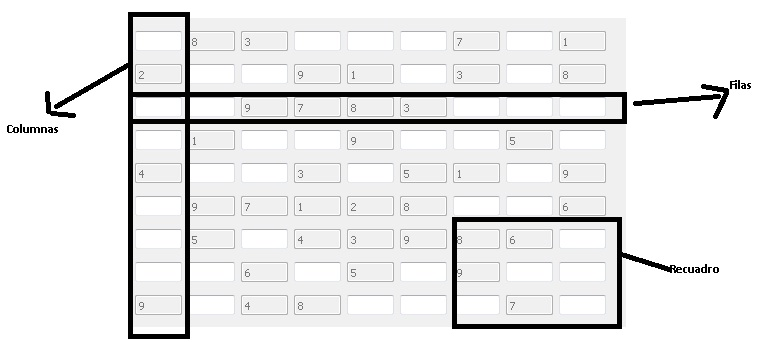
\includegraphics[width=.60\textwidth]{./imagenes/6.jpg}
\caption{Estructuras básicas}
\label{Estructuras básicas}
\end{center}
\end{figure}


El objetivo del juego es completar el tablero (inicialmente con unas pocas casillas llenas) con los números indicados. 
Las reglas son: En cada columna no puede existir  repiticiones del mismo número, lo mismo en cada fila y en cada recuadro.
Un recuadro es un grupo de 9 casillas, hay 9 recuadros en el tablero.

\newpage
\begin{figure}[htbp]
\begin{center}
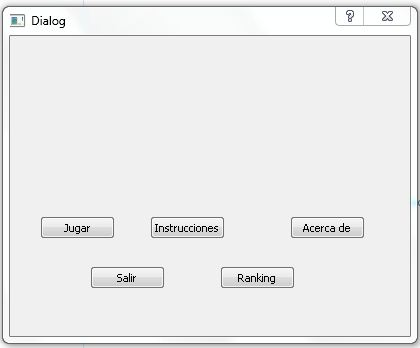
\includegraphics[width=.60\textwidth]{./imagenes/1.jpg}
\caption{Ventana Principal}
\label{Ventana Principal}
\end{center}
\end{figure}
El usuario comienza en la ventana principal, donde puede escoger cualquiera de las opciones presentadas. Para empezar el juego, le deberá dar click en jugar.

\newpage
\begin{figure}[htbp]
\begin{center}
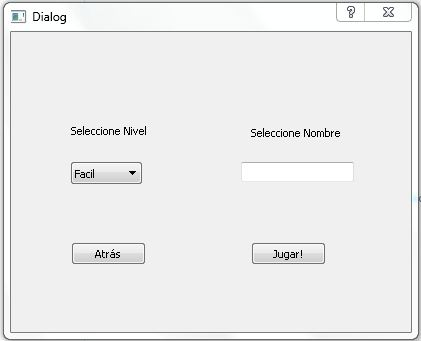
\includegraphics[width=.60\textwidth]{./imagenes/2.jpg}
\caption{Ventana de Elección}
\label{Ventana de Elección}
\end{center}
\end{figure}
En esta ventana ingresará la dificultad y el nombre. La dificultad esta dada por un número (dado por la dificultad), que al ingresar al algoritmo es el la cantidad de números que se va a extraer por recuadro.

\newpage
\begin{figure}[htbp]
\begin{center}
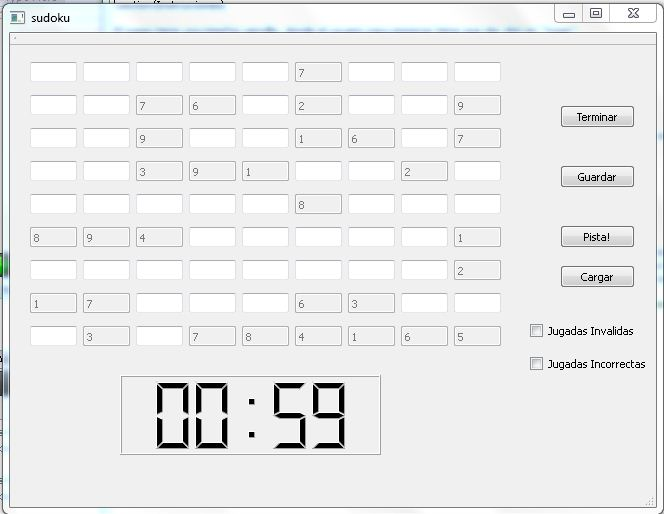
\includegraphics[width=.60\textwidth]{./imagenes/3.jpg}
\caption{Ventana del Juego}
\label{Ventana del Juego}
\end{center}
\end{figure}

\begin{figure}[htbp]
\begin{center}
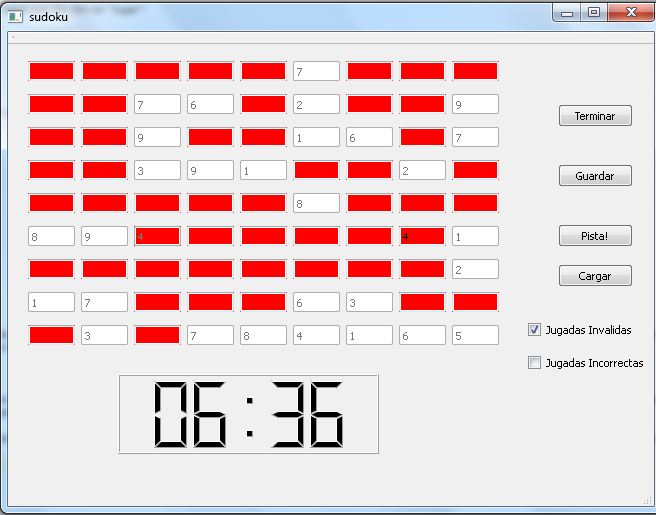
\includegraphics[width=.60\textwidth]{./imagenes/4.jpg}
\caption{Jugadas Inválidas}
\label{Jugadas Inválidas}
\end{center}
\end{figure}


Ya en esta ventana el usuario puede jugar. Se recuerda que no se podrá acceder a la funcionalidad del ranking si se carga una partida , se usa la funcionalidad pista o se usa las funcionalidades Jugadas Inválidas e Incorrectas.

Al presionar el boton pista una casilla vacía tomará el valor correcto segun la solución del sudoku.

Al acceder a la funcionalidad de las jugadas inválidas, se verifica el estado actual del sudoku, y jugadas incorrectas se verifica los números incorrectos con respecto a la solución del sudoku.

El reloj en la parte inferior indica el tiempo, el cuál es el puntaje del jugador.







\chapter{Funcionalidades}
\section{Ranking}
Esta funcionalidad es accecida mediante la primera pantalla del programa, dandole click al botón ranking.
\begin{figure}[htbp]
\begin{center}
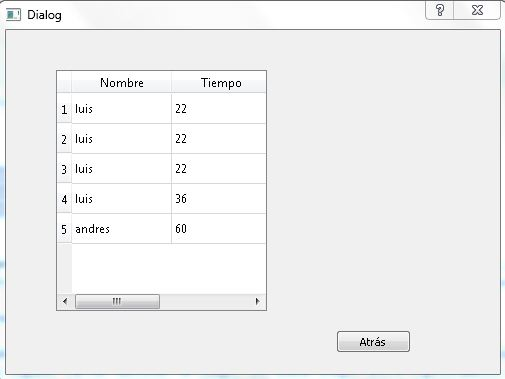
\includegraphics[width=.60\textwidth]{./imagenes/5.jpg}
\caption{Pantalla Ranking}
\label{Pantalla Ranking}
\end{center}
\end{figure}


Esta funcionalidad se la llevo a cabo usando un widget en Qt especial, que nos permitió armar una tabla con los nombres de los jugadores. El ranking es guardado en un archivo de texto ranking.txt, y es cargado en tiempo real a la tabla. Al finalizar el juego de forma satisfactoria el nombre del jugador y el puntaje (número de segundos) son guardados en este archivo.


\section{Guardar y Cargar }
Esta funcionalidad es accecida mediante la pantalla del juego del programa, haciendo click en guardar o cargar.


Esta funcionalidad funciona de forma que guarda el sudoku presente en pantalla, en un archivo .txt cifrado en un tipo de código binario.
La funcionalidad cargar carga desde este mismo archivo el sudoku, y lo pone en pantalla. Nótese que si se usa cargar, no se podrá acceder a la opción de ranking
\begin{figure}[htbp]
\begin{center}
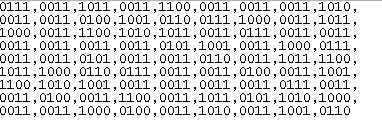
\includegraphics[width=.60\textwidth]{./imagenes/7.jpg}
\caption{Archivo Cifrado}
\label{Archivo Cifrado}
\end{center}
\end{figure}
\chapter{Conclusiones}
\section{Responsabilidades Cumplidas y Conclusiones}
Responsabilidades:
\begin{itemize}
\item[Luis Vasquez] Interfaz Gráfica, funcionalidad de Guardar y Cargar, conectividad entre la parte lógica y la parte visual, Manual en Látex
\end{itemize}
\begin{itemize}
\item[Luis Caviedes]Generación del Sudoku, Niveles, Ranking y generación de pistas.
\end{itemize}

Conclusiones:
El proyecto se puede mejorar de muchas maneras, pero lo principal es la interfaz gráfica, que por cuestiones de tiempo no se pudo completar de la manera deseada, solo se la hizo para que la parte funcional corra. Estos errores se corregirán el segundo proyecto.

\end{document}